\documentclass{article}\usepackage[]{graphicx}\usepackage[]{xcolor}
% maxwidth is the original width if it is less than linewidth
% otherwise use linewidth (to make sure the graphics do not exceed the margin)
\makeatletter
\def\maxwidth{ %
  \ifdim\Gin@nat@width>\linewidth
    \linewidth
  \else
    \Gin@nat@width
  \fi
}
\makeatother

\definecolor{fgcolor}{rgb}{0.345, 0.345, 0.345}
\newcommand{\hlnum}[1]{\textcolor[rgb]{0.686,0.059,0.569}{#1}}%
\newcommand{\hlsng}[1]{\textcolor[rgb]{0.192,0.494,0.8}{#1}}%
\newcommand{\hlcom}[1]{\textcolor[rgb]{0.678,0.584,0.686}{\textit{#1}}}%
\newcommand{\hlopt}[1]{\textcolor[rgb]{0,0,0}{#1}}%
\newcommand{\hldef}[1]{\textcolor[rgb]{0.345,0.345,0.345}{#1}}%
\newcommand{\hlkwa}[1]{\textcolor[rgb]{0.161,0.373,0.58}{\textbf{#1}}}%
\newcommand{\hlkwb}[1]{\textcolor[rgb]{0.69,0.353,0.396}{#1}}%
\newcommand{\hlkwc}[1]{\textcolor[rgb]{0.333,0.667,0.333}{#1}}%
\newcommand{\hlkwd}[1]{\textcolor[rgb]{0.737,0.353,0.396}{\textbf{#1}}}%
\let\hlipl\hlkwb

\usepackage{framed}
\makeatletter
\newenvironment{kframe}{%
 \def\at@end@of@kframe{}%
 \ifinner\ifhmode%
  \def\at@end@of@kframe{\end{minipage}}%
  \begin{minipage}{\columnwidth}%
 \fi\fi%
 \def\FrameCommand##1{\hskip\@totalleftmargin \hskip-\fboxsep
 \colorbox{shadecolor}{##1}\hskip-\fboxsep
     % There is no \\@totalrightmargin, so:
     \hskip-\linewidth \hskip-\@totalleftmargin \hskip\columnwidth}%
 \MakeFramed {\advance\hsize-\width
   \@totalleftmargin\z@ \linewidth\hsize
   \@setminipage}}%
 {\par\unskip\endMakeFramed%
 \at@end@of@kframe}
\makeatother

\definecolor{shadecolor}{rgb}{.97, .97, .97}
\definecolor{messagecolor}{rgb}{0, 0, 0}
\definecolor{warningcolor}{rgb}{1, 0, 1}
\definecolor{errorcolor}{rgb}{1, 0, 0}
\newenvironment{knitrout}{}{} % an empty environment to be redefined in TeX

\usepackage{alltt}
\usepackage{amsmath} %This allows me to use the align functionality.
                     %If you find yourself trying to replicate
                     %something you found online, ensure you're
                     %loading the necessary packages!
\usepackage{amsfonts}%Math font
\usepackage{graphicx}%For including graphics
\usepackage{hyperref}%For Hyperlinks
\usepackage[shortlabels]{enumitem}% For enumerated lists with labels specified
                                  % We had to run tlmgr_install("enumitem") in R
\hypersetup{colorlinks = true,citecolor=black} %set citations to have black (not green) color
\usepackage{natbib}        %For the bibliography
\setlength{\bibsep}{0pt plus 0.3ex}
\bibliographystyle{apalike}%For the bibliography
\usepackage[margin=0.50in]{geometry}
\usepackage{float}
\usepackage{multicol}

%fix for figures
\usepackage{caption}
\newenvironment{Figure}
  {\par\medskip\noindent\minipage{\linewidth}}
  {\endminipage\par\medskip}
\IfFileExists{upquote.sty}{\usepackage{upquote}}{}
\begin{document}

\vspace{-1in}
\title{Lab 10 -- MATH 240 -- Computational Statistics}

\author{
  Jeremy Artiga \\
  Colgate University  \\
  {\tt jartiga@colgate.edu}
}

\date{}

\maketitle

\begin{multicols}{2}

\begin{abstract}
In this lab, we will simulate data based on statistics provided by Gallup Polls concerning the satisfaction of the US politically to figure out how exactly Gallup derived their confidence interval and margin of errors while I've. This will involve the use of re-sampling and \texttt{R} simulations to illustrate how the confidence interval and margin of error changes with differences in probability and sample size.
\end{abstract}

\section{Introduction}
Statistical analysis of proportions, such as those found in public opinion polls, relies heavily on understanding the margin of error and confidence intervals. The margin of error reflects the uncertainty in a sample estimate, and is influenced by numerous factors. In this lab, we will explore how changes in sample size and probability affect the margin of error in statistical analyses of proportions and how these statistics are modeled in real life using data from Gallup's \citep{gallup2025} polls on the satisfaction of the current US well-being with emphasis on the use of simulations and re-sampling with \texttt{R}'s tidyverse \citep{tidyverse}!

\section{Methodology}
\subsection{Simulations}
Assuming the probability calculated by the Gallup polls to be true (concerning the satisfactions of the US political state), we will start by conducting 10000 simulations of the Gallup polls under the assumptions that $p = 0.39$ and $n = 1004$ (statistics derived from the Gallup study). We will take the range of this data and calculate a margin of error. We will also repeat this with $n= 2008$ to see how these statistics change. \\

As seen in Figure \hyperref[fig1]{1}, the distribution of the proportions calculated in the simulations appear to be normal, with a peak at the probability 0.39. This is also supported by the calculated range (middle 95\%) of the data, which is at 0.42-0.361. The margin of error calculated for this simulations sits at $\approx 3\%$, which is one lower than the margin of error calculated by the Gallup.

\begin{figure}[H]
  \centering
  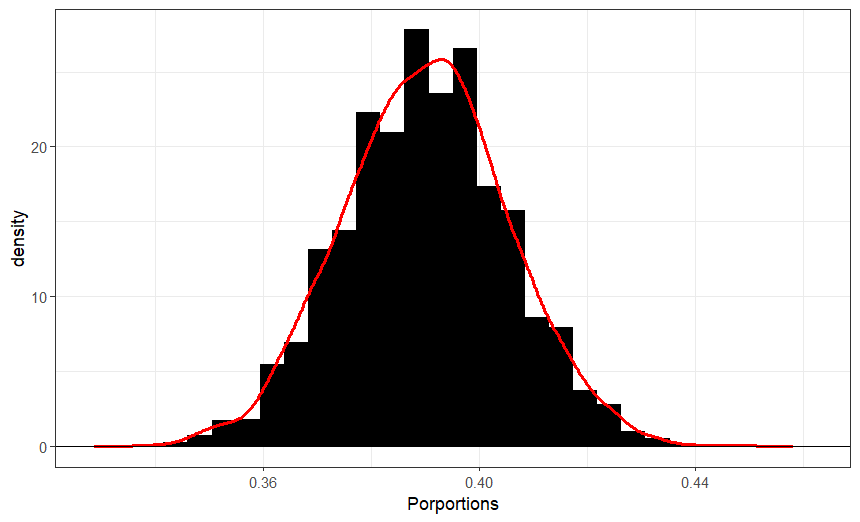
\includegraphics[width=\columnwidth]{sample1004.png}
  \caption{Distribution of 10000 Poll Simulations with Sample Size $n = 1004$, and Probability $p = 0.39$}
  \label{fig1}
\end{figure}

As seen in Figure \hyperref[fig2]{2}, when we double the sample size under the same assumptions (i.e. probability), we get a much cleaner normal distribution with a peak also centered at 0.39. The range in this data spans from 0.411 to 0.369, which is shorter than the $n = 1004$ distribution. Since our range is shorter, our margin of error was also reduced down to $\approx 2\%$, which matches what Gallup approximated.

\begin{figure}[H]
  \centering
  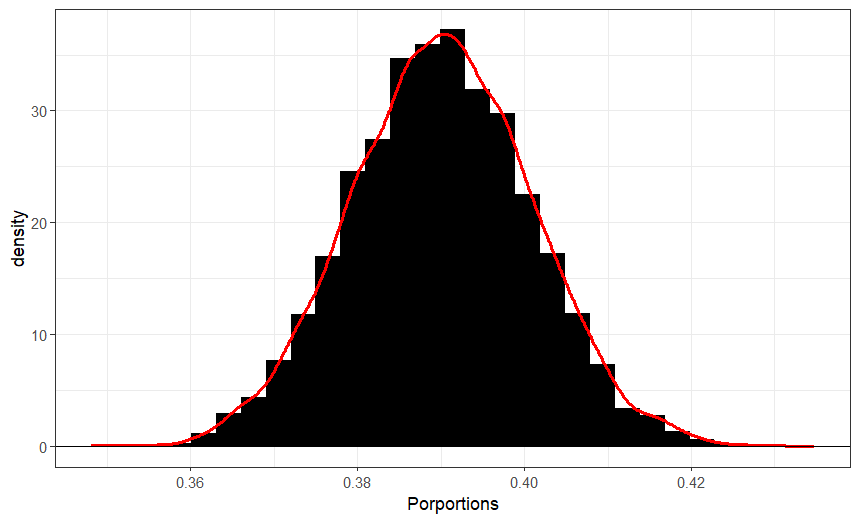
\includegraphics[width=\columnwidth]{sample2008.png}
  \caption{Distribution of 10000 Poll Simulations with Sample Size $n = 2008$, and Probability $p = 0.39$}
  \label{fig2}
\end{figure}

As we can see with simulations, by increasing the sample size, we are able to obtain a much narrower range with a lower margin of error for given data. This essentially illustrates the power of the sample size effect!

\subsection{Resampling}
To further validate our margin of error estimate, we will perform re-sampling with the same data used by the Gallup poll in their study. Specifically, we took 1000 re-samples (with replacement) from the original set of responses, each of size $n = 1004$. Focusing on only the responses with a "yes" output, we performed the same range and margin of erro calculations as we did in our simulations . This approach mirrors how poll results might vary in repeated sampling under the same conditions. \\

As illustrated in Figure \hyperref[fig3]{3}, the resulting distribution of proportions is approximately normal, with a peak centered near 0.39. The 95\% interval of these simulated proportions range from approximately 0.36 to 0.42. From this, we calculate a margin of error of $\approx 3\%$, which aligns closely with the margin of error reported in the original Gallup poll.

\begin{figure}[H]
  \centering
  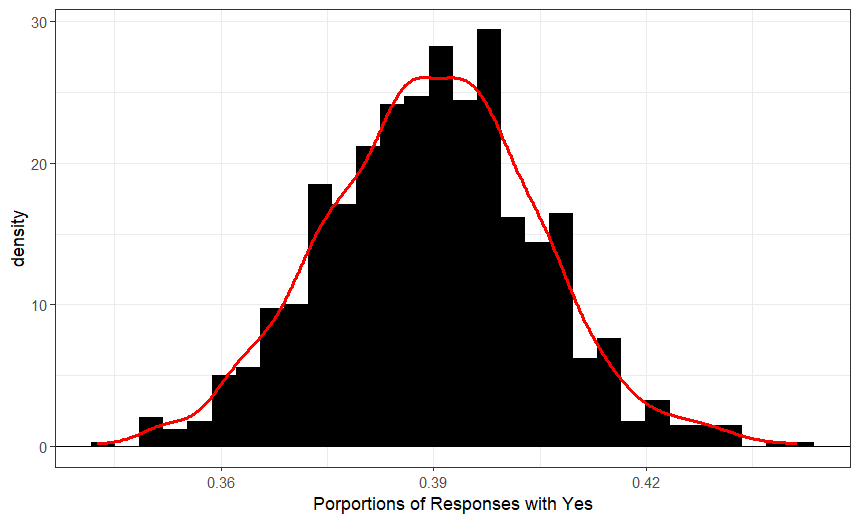
\includegraphics[width=\columnwidth]{GallupYes.png}
  \caption{Distribution of Gallup Poll Respondents who Answered "Yes"}
  \label{fig3}
\end{figure}

This method of re-sampling demonstrates how the margin of error originates in from sampling variability and reinforces the concept of larger spreading in sample proportions yield higher uncertainty in our estimate. The use of re-sampling thus offers a practical and intuitive approach to assessing confidence in survey data.

\subsection{How Does Error Change Over Probability and Sample Size?}
With the way we've seen the confidence interval (range) and margin of error change with alterations in our sample size, that begs an interesting question, how does confidence interval and margin of error change with alterations in probability and sample size? \\
To illustrate this, we will need to create a plot which illustrates the relationship between probability and sample size with respect to confidence interval and margin of error. Since margin of error is directly correlated to the confidence interval, we will use the margin of error to illustrate the relationship between probability and sample size. To accomplish this, we simulated various margin of errors across $p = \{0.01, 0.02, ..., 0.99 \}$ and $n = \{100, 110, ..., 3000 \}$ where p is defined as probability and n is defined as our sample size. The results of our simulations our illustrated in Figure \hyperref[fig4]{4} below. 

\begin{figure}[H]
  \centering
  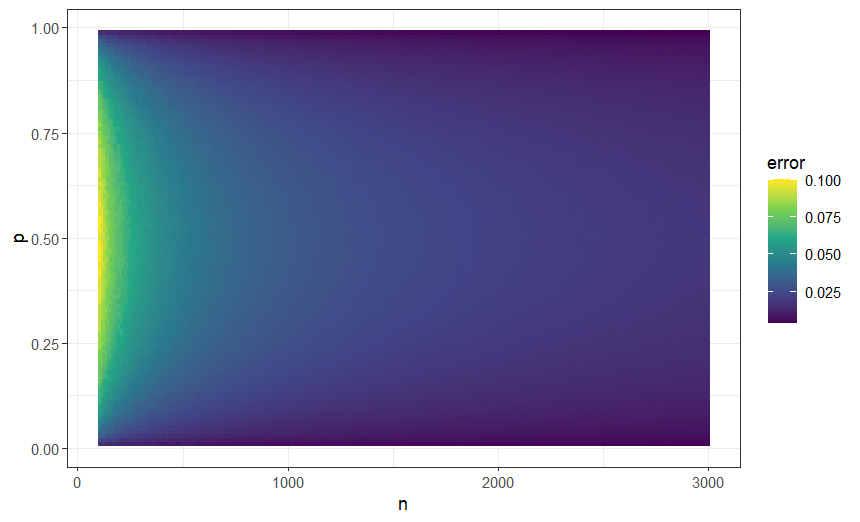
\includegraphics[width=\columnwidth]{Simulationraster.png}
  \caption{Simulated Margin of Error in terms of Probability and Sample Size}
  \label{fig4}
\end{figure}

As seen by the raster plot in Figure \hyperref[fig4]{4}, we can see that as $n$ increases, our error becomes much smaller for a constant $p$. This means that as our sample size increases, our margin of error decreases under the assumption our probability doesn't change. In terms of $p$ however, we see that as $p$ approaches the mid point of the interval [0,1], our error becomes much larger (and vice-versa) for a constant $n$. In other words, our margin of error becomes much larger as we approach probability .50 under the assumption that sample size of constant.

This figure validates our previous findings of the sample size effect as it illustrates how increases in sample sizes with correlates with a decrease in the margin of error (i.e. the sample size effect) and decrease in variability . It also describes how probability has a hand in influencing the margin of error and confidence intervals (in the binomial distribution), as values that approach a probability of 0.50 end up maximizing the margin of error, which also implies a wider confidence interval.

\subsection{The Actual Margin Of Error}
Up until now, we've been using simulations and re-sampling to calculate our margin of errors, however, we are able to calculate the actual margin of errors using Wilson's margin of error formula. Using this formula yields greater accuracy in the calculations of the margin of errors for our data, if we can show that the raster plot for Wilson's margin of errors is very similar to our simulations raster plots, then our findings are validated! \\
By using the same process to generate the raster plots, we calculated Wilson's margin of error across $p = \{0.01, 0.02, ..., 0.99 \}$ and $n = \{100, 110, ..., 3000 \}$ where p is defined as probability and n is defined as our sample size. The results of our simulations our illustrated in Figure \hyperref[fig5]{5} below. 

\begin{figure}[H]
  \centering
  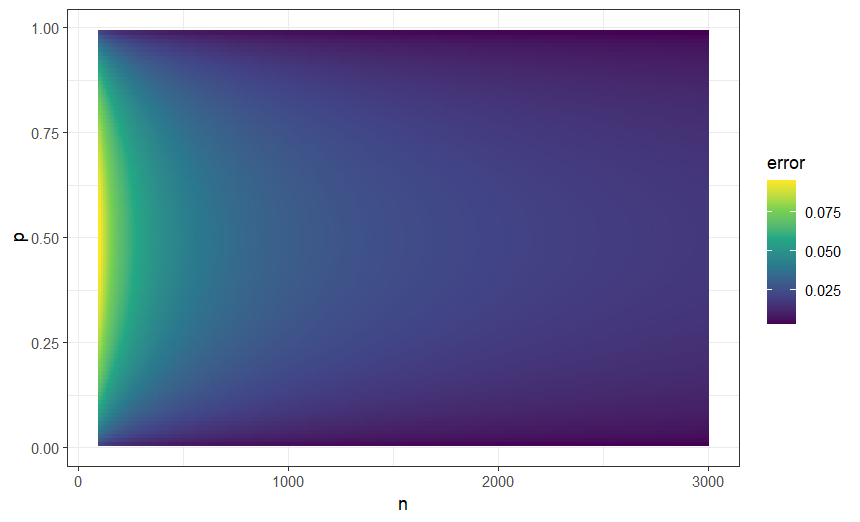
\includegraphics[width=\columnwidth]{Wilsons.png}
  \caption{Wilson's Margin of Error in terms of Probability and Sample Size}
  \label{fig5}
\end{figure}

As we can see, the raster plots in Figures \hyperref[fig4]{4} and \hyperref[fig5]{5} look practically identical, which reinforces our findings concerning the relationship between the confidence interval and margin of error with probability and sample size!

\section{Discussion}
This lab illustrated that sample size and probability play a crucial role in the accuracy of survey estimates. Increasing the sample size reduces the margin of error, making results more reliable. As we've seen in the simulations and use of the Gallup polls, the increase of the sample size has greatly reduced the margin of error and variance for the plotted distribution, which also allowed us to validate the Gallup's poll results. \\
Additionally, we also found that the probability of an outcome affects the margin of error. When the probability is around 0.5, the margin of error is larger, meaning results are more uncertain. This should be considered when designing surveys. \\
Using Wilson’s margin of error formula also helps ensure accuracy, validating the results of our simulations. These findings highlight the importance of sample size and probability in creating more reliable surveys and improving decision-making.




%%%%%%%%%%%%%%%%%%%%%%%%%%%%%%%%%%%%%%%%%%%%%%%%%%%%%%%%%%%%%%%%%%%%%%%%%%%%%%%%
% Bibliography
%%%%%%%%%%%%%%%%%%%%%%%%%%%%%%%%%%%%%%%%%%%%%%%%%%%%%%%%%%%%%%%%%%%%%%%%%%%%%%%%
\begin{tiny}
\bibliography{bib}
\end{tiny}
\end{multicols}

\end{document}
